\section{Product Overview}
In this product we want to recreate the old SNAKE game from the Nokia 3310 phone. The game will be created using an Nokia 5110 48 x 84 LCD matric display \cite{NokiaDisplay}; the same model that was used in the original Nokia 3310. The user will use a matrix keyboard to control the snake in the same way as in the original game. The system is driven by an ATMEGA 2560 that will read the user input, do the game calculations, and draw the game onto the display. In our version of snake, we are also keeping a highscore list. This highscore is saved in the non-volatile flash memory of the ATMEGA 2560 to ensure that it is persisted even if the power for the ATMEGA is off.

\section{System Description}
In figure \ref{ProductComponents} the product can be seen. The red square shows the Arduino board containing the ATMEGA 2560 microcontroller. This is connected to the matrix keyboard highlighted in the blue square, and the Nokia display indicated with green. 

\begin{figure}[H]
	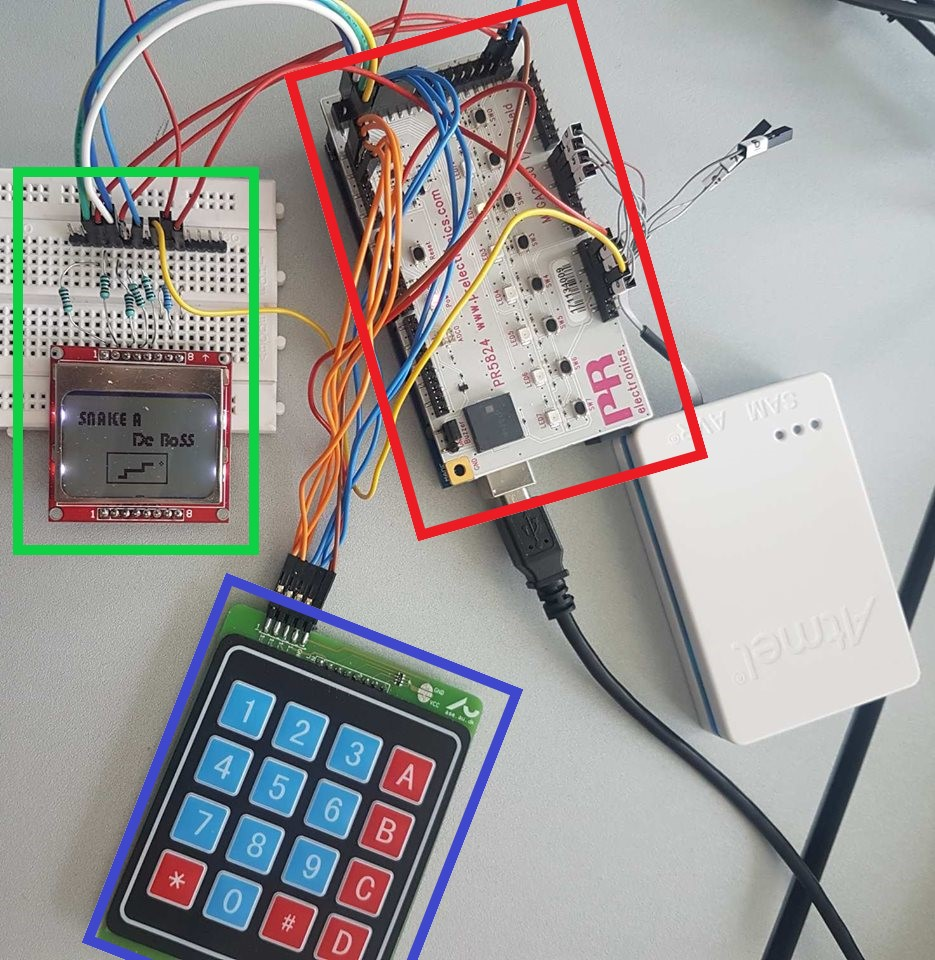
\includegraphics[width=12cm]{ProductComponents}
	\centering
	\caption{Picture of the setup}
	\label{ProductComponents}
\end{figure}


\subsection{Block Definition Diagram}

\subsection{Internal Block Diagram}
